%% ----------------------------------------------------------------------------
% BIWI SA/MA thesis template
%
% Created 09/29/2006 by Andreas Ess
% Extended 13/02/2009 by Jan Lesniak - jlesniak@vision.ee.ethz.ch
%% ----------------------------------------------------------------------------
\documentclass[pdftex,11pt,openright,headsepline]{book}

\usepackage{paralist}		% List environment
\usepackage{color}		% For colored text
\usepackage{times}
\usepackage{amsfonts}		% Additional math fonts
\usepackage{amsmath}		% Math symbols
\usepackage{latexsym}
\usepackage{graphicx}		% For including images
%\usepackage{listings}		% If listings are needed
%\usepackage{mydefs}		% Some of our own definitions
% \usepackage{wrapfig}		% To wrap images
% \usepackage{algorithmic}	% Nice algorithm environment
% \usepackage{algorithm}
\usepackage{fancyhdr}		% Produce the nice header
\usepackage{fullpage}           % Use the full page
\usepackage{url}
\usepackage{amssymb}
\usepackage{mathtools}
\usepackage{setspace}
\doublespacing
\usepackage{xspace}
\usepackage{etoolbox}

\newcommand{\littleo}{o\mathopen{}}
\newcommand{\bigO}{O\mathopen{}}


\newcommand\foreign[1]{\emph{#1}}
\newcommand\eg{\foreign{e.g.}\xspace}
\newcommand\ie{\foreign{i.e.}\xspace}
\newcommand\vs{\foreign{vs.}\xspace} 
\newcommand\apriori{\textit{a priori}\xspace}
\newcommand\aposteriori{\textit{a posteriori}\xspace}

%real line
\newcommand*\R{\mathbb{R}}

% \diff : differential operator
\newcommand{\diff}{\mathop{\mathrm{{}d}}\mathopen{}}


% \vec, \mat : typesetting vectors and matrices
\renewcommand{\vec}[1]{\ensuremath{\boldsymbol{#1}}}
\newcommand{\mat}[1]{\ensuremath{\boldsymbol{#1}}}


% \transpose, adjoint : transpose, adjoint of a matrix/operator
\newcommand{\transpose}[1]{\ensuremath{#1^{T}}\xspace}
\newcommand{\adjoint}[1]{\ensuremath{\transpose{#1}}\xspace}

% \crossprod : typesetting cross product
\newcommand\crossprod{\mathbin{\times}}



% \funop : define symbols representing functions, for correctly
% handling spacing
%\newcommand\funop[1]{\mathop{{}#1}}
\newcommand\funop[1]{\mathop{{}#1}}

\newcommand\LHS{\mathrm{L.H.S.}}
\newcommand\RHS{\mathrm{R.H.S.}}

%variables
\newcommand*\x{\ensuremath{\vec{x}}\xspace}
\newcommand*\dx{\diff \x}

\newcommand*\p{\ensuremath{\vec{p}}\xspace}


\newcommand*\y{\ensuremath{\vec{y}}\xspace}
\newcommand*\dy{\diff \y}


\newcommand*\dt{\diff t}

\newcommand*\dl{\diff l}

\newcommand*\du{\diff u}
\newcommand*\dv{\diff v}


\newcommand*\PSF{\ensuremath{K}\xspace}
\newcommand*\fPSF{\funop{\PSF}}


\newcommand*\PhotonFlux{\ensuremath{\Phi}\xspace}
\newcommand*\fPhotonFlux{\funop{\PhotonFlux}}

\newcommand\ConvSymbol{*}
\newcommand\conv{\mathbin{\ConvSymbol}}

\newcommand*\dirac{\delta}
\newcommand{\fdirac}[1]{\funop{\delta_{#1}}}

\newcommand*\Pixel{\ensuremath{\mathcal{P}}\xspace}
\newcommand*\T{\ensuremath{T}}
\newcommand*\TInterval{\ensuremath{\intervalcc{0}{T}}\xspace}

% This new command ensure right spacing
\newcommand{\interval}[4]{\mathopen{#1}#2 \mathclose{}\mathpunct{}, #3\mathclose{#4}} 
\newcommand{\intervalcc}[2]{\interval{[}{#1}{#2}{]}} % interval close close : [ , ]

\newcommand*\eqend{\quad .}
\newcommand*\eqcont{\quad ,}

\newcommand*\m{\vec{m}}
\newcommand*\matS{\mat{\Sigma}}

\newcommand*\cma{\textit{CMA-ES} }
\newcommand*\dic{\textbf{dictionary} }

\newcommand{\nll}{\mathop{\mathrm{{}nll}}\mathopen{}}

\newcommand*\w{\ensuremath{\vec{w}}\xspace}
\newcommand*\vb{\ensuremath{\vec{b}}\xspace}
\newcommand*\vv{\ensuremath{\vec{v}}\xspace}

\setlength{\headsep}{10mm}


% Change the appearance of the header. Here \MakeUppercase is hard-coded, so renewing this command allows to elegantly change the header appearance.
\renewcommand{\MakeUppercase}{\scshape}

% Set the headings' appearance in the ``fancy'' pagestyle
\fancyhead{}
\fancyhead[RO, LE]{\leftmark}
\fancyfoot{}
\fancyfoot[RO, LE]{\thepage}



% The first pages shall be empty, even no page numbering 
\begin{document}
\pagestyle{empty} % even no page number

\fancypagestyle{plain}{
  \renewcommand{\headrulewidth}{0.0pt}
  \fancyfoot{}
  \fancyhead{}
}


% Title page, modify accordingly 
%% ----------------------------------------------------------------------------
% BIWI SA/MA thesis template
%
% Created 09/29/2006 by Andreas Ess
% Extended 13/02/2009 by Jan Lesniak - jlesniak@vision.ee.ethz.ch
%% ----------------------------------------------------------------------------

\begin{titlepage}

\thispagestyle{empty}

\fancypagestyle{empty}{
\lhead{
\includegraphics[height=1.5cm]{images/ethlogo_black}}
\renewcommand{\headrulewidth}{0.0pt}
\rhead{\vspace*{-0.2cm}
\includegraphics[height=1.4cm]{images/cvl_varcity_2013_horiz}}
\fancyfoot{}
}



\vspace*{2cm}
\begin{center}
\Huge{\textbf{Semi-supervised learning using Total variation for biomedical image segmentation}\\}
\LARGE{\textbf{}\\[1cm]}

\large{Master Thesis\\[0.8cm]}
\LARGE{Prateek Purwar\\}
\normalsize{Department of Electrical Engineering and Information Technology}
\end{center}

\begin{center}
 


% \begin{center}
% \begin{tabular}{ll}
% \multirow{2}{*}{
\includegraphics[height=1cm]{images/biwi_logo}} & Computer Vision Laboratory\\ 
% & ETH Zurich
% \end{tabular}
%  \end{center}

\end{center}


\vfill
\begin{center}
\begin{tabular}{ll}
\Large{\textbf Advisor:} & \Large{Dr. Gregory Paul}\\
\Large{\textbf Supervisor:} & \Large{Prof.~Dr.~Orcun Goksel}\\
% 			    & \small{Computer Vision Laboratory}\\
% 			    & \small{Department of Information Technology and Electrical Engineering}\\
\end{tabular}
\end{center}



\end{titlepage}

\cleardoublepage

%% ----------------------------------------------------------------------------
% BIWI SA/MA thesis template
%
% Created 09/29/2006 by Andreas Ess
% Extended 13/02/2009 by Jan Lesniak - jlesniak@vision.ee.ethz.ch
%% ----------------------------------------------------------------------------

\newpage
\vspace{3cm}

\chapter*{Abstract}



% Input here any acknowledgements
%% ----------------------------------------------------------------------------
% BIWI SA/MA thesis template
%
% Created 09/29/2006 by Andreas Ess
% Extended 13/02/2009 by Jan Lesniak - jlesniak@vision.ee.ethz.ch
%% ----------------------------------------------------------------------------
\chapter*{Acknowledgements}
I would like to acknowledge the support of my Semester Thesis advisor Dr. Gregory Paul, Post-Doc. at Computer Vision Laboratory at ETH. He consistently steered me in the right direction whenever he thought I needed it. I would sincerely thank Denis Samuylov, who helped with implementation and coding at each step of my thesis. 


\cleardoublepage
\newpage

% % Chapter-pages etc. use the ``plain'' pagestyle - since we don't want to have a heading at all at chapter-pages, redefine plain accordingly. Don't forget the page number. 
\fancypagestyle{plain}{
  \renewcommand{\headrulewidth}{0.0pt}
  \fancyfoot{}
  \fancyfoot[RO, LE]{\thepage}
  \fancyhead{}
}

\pagestyle{fancy}
\pagenumbering{Roman}

\let\cleardoublepage\clearpage
% Insert table of contents
\tableofcontents

% Insert list of figures
\listoffigures

\newpage

\pagenumbering{arabic}

%% ----------------------------------------------------------------------------
% Actual text comes here - defer it to other files and use \input{bla.tex}, ..
%% ----------------------------------------------------------------------------
%% ----------------------------------------------------------------------------
% BIWI SA/MA thesis template
%
% Created 09/29/2006 by Andreas Ess
% Extended 13/02/2009 by Jan Lesniak - jlesniak@vision.ee.ethz.ch
%% ----------------------------------------------------------------------------


\chapter{Introduction}

\section{Focus of this Work}
The task of image segmentation into binary classes is very useful in different cases in biomedical tasks. It can be used for detection of diseases, shape analysis etc. The methods to solve the segmentation problem has evolved among two lines: 1) level of interaction: from semi-interactive to fully automatic, and 2) level of classification: pixels to complete images. Nowadays, with the use of fully-convolutional networks, the segmentation can be obtained for complete image. This helps in using the local as well as contextual information for segmentation and significantly, improves performance in terms of speed. This speeds up the task of segmentation especially for huge images in cases such as electron microscopic images, 3-D images etc. Currently, the benchmark performance in terms of accuracy is achieved by the use of deep-neural networks. Deep neural networks such as U-net are specially designed for task of segmentation.
\par The only limitation with use of convolutional neural networks is need of huge training data for training these networks. Earlier networks solved the segmentation problem by training a neural network for classifying each pixel into corresponding classes. These networks were trained using a patch around training pixels. These networks faced problem of speed for cases of huge images where we have to run neural network for total number of pixels. Also, we get limited by the local information provided by the patch surrounding training pixels. This problem gets solved by use of fully-convolutional networks which produces segmentation for the whole input image at once. But we require fully annotated ground truth images for training such networks i.e. label for each pixel in the input image.  

\subsection{Dataset}
The dataset or the images which we are trying to segment are electron microscopic images. The microscopic images are huge in size i.e. order of 450x512x512. This poses a huge problem of creating a fully annotated ground truth. In addition to huge size of images, the images may contain multiple instances of objects to be annotated. For example, the liver tissue contain many vesicles. This makes the task of creating ground truth dataset hard and time consuming. The argument that the annotated dataset can be used again as for object segmentation in natural images also fails here as the objects to be segmented in microscopic images differ completely. This inhibits the experts to invest time to create fully annotated dataset. Further, the manual annotations for a single microscopic image may differ for each expert or even different for a single expert. This arise due to arbitrary shapes and sizes of objects to be segmented. This influences us to design a approach with semi-interactivity possible so that the experts can modify/add information according to their needs. In summary, we have to consider following scenarios before developing a method to solve our segmentation task, 
\begin{itemize}
\item High variability between images: The images to be segmented may be entirely different for example of liver and neuron tissue. It is not same as case for natural images.
\item High variability between objects to segment: The objects to be segmented may differ completely from being smooth (round vesicles) to branched (neurons)
\item High variability between goals: 
\end{itemize}

Therefore, we plan to use an approach that can be modified easily to new images/objects to be segmented. This influences us to use hybrid of data and model driven approach. We decided to use an semi-supervised approach using Maximum-aposteriori inference. The idea is to propagate segmentation label from labeled to unlabeled pixels using an prediction model and a prior, as shown in figure 1.1. The prediction model and prior are combined using Variational image processing methods. As shown in figure 1.1, this can be used to generate segmentation or can be used to train other prediction model if needed.
We can observe that the limitation on availability of fully annotated ground truth images inspires us to observe the trade-off between partially labeled data and accuracy of segmented images. This will enable the experts to use their annotation budget i.e. the pixels labeled by experts for training, efficiently giving best results. In addition, we observe effect of different ways of introducing maximum-likelihood and different regularisation parameter for total variation.

\section{Thesis Organization}




% %% ----------------------------------------------------------------------------
% BIWI SA/MA thesis template
%
% Created 09/29/2006 by Andreas Ess
% Extended 13/02/2009 by Jan Lesniak - jlesniak@vision.ee.ethz.ch
%% ----------------------------------------------------------------------------
\newpage
\chapter{Related Work}

\let\cleardoublepage\clearpage
% %% ----------------------------------------------------------------------------
% BIWI SA/MA thesis template
%
% Created 09/29/2006 by Andreas Ess
% Extended 13/02/2009 by Jan Lesniak - jlesniak@vision.ee.ethz.ch
%% ----------------------------------------------------------------------------
\newpage
\chapter{Method for image segmentation}
\section{Bayesian Formulation}
We model our image segmentation problem as a Bayesian inference problem.
Let us cosider an observed image, \mat{I} and labeled or segmented groud truth, \mat{S}, the joint probabilty can be defined as:
\begin{equation*}
\p(\mat{I}, \mat{S}) = \p(\mat{S}) \p(\mat{I}|\mat{S}) \eqcont
\end{equation*}
and applying Bayes theorem,
\begin{align*}
\p(\mat{S}|\mat{I}) \, & = \frac{{\p(\mat{S}) \p(\mat{I}|\mat{S})}{\p(\mat{I})}}
						& \alpha {\p(\mat{S}) \p(\mat{I}|\mat{S})}
\end{align*}
The left hand side is the probability of \mat{S} given the image \mat{I}, is called the
posterior probability. \p\mat{S} is the prior probability of \mat{S}. The Maximum a posteriori (MAP) estimate, $\mat{S^*}$ can be calculated as follow:
\begin{equation*}
\mat{S^*} = \arg\max_{\S}{\p(\mat{S}) \p(\mat{I}|\mat{S})} \eqend
\end{equation*}

The above problem can as well be stated as an energy minimization problem by
writing Equation 2.3 in terms of energy:
\begin{align*}
\funop{E}(\mat{S}) &= − \log(\p(\mat{I}, \mat{S}))

&= − \log(\p(\mat{I}|\mat{S})) − \log(\p(\mat{S}))
&= \funop{E_d}(\mat{I}, \mat{S}) + \funop{E_r} (\mat{S})
\end{align*}
The total energy, \funop{E}, that we want to minimize can be considered as linear combination of data term, \funop{E_d} and prior term (or regularization), \funop{E_r}. This modifies calculating MAP estimate to:
\begin{equation*}
\mat{S^*} = \arg\min_{\S}{\funop{E_d}(\mat{I}, \mat{S}) + \funop{E_r} (\mat{S})} \eqend
\end{equation*}

\section{Data energy term or Maximum likelihood cost function}
Explain different cost functions

\section{Prediction models}
\subsection{Random Forests}
Explain random forests
\subsection{Convolutional Neural Networks}
Neural networks
Explain transfer learning also.

\subsection{Prior energy term: Variational Image Processing}
Explain total variation regularisation term.


\chapter{Implementation}
\section{Solving variational problem using ASB}
\section{Random Forest}
\section{CNN using VGG-16}
% %% ----------------------------------------------------------------------------
% BIWI SA/MA thesis template
%
% Created 09/29/2006 by Andreas Ess
% Extended 13/02/2009 by Jan Lesniak - jlesniak@vision.ee.ethz.ch
%% ----------------------------------------------------------------------------
\newpage
\chapter{Experiments and Results}


%% ----------------------------------------------------------------------------
% BIWI SA/MA thesis template
%
% Created 09/29/2006 by Andreas Ess
% Extended 13/02/2009 by Jan Lesniak - jlesniak@vision.ee.ethz.ch
%% ----------------------------------------------------------------------------
\newpage
\chapter{Training CNNs using fully annotated segmentation masks}
Nowadays, the CNNs have evolved with great speed to solve major problems in classical computer vision scenario. Instead of using classical image processing filters, the CNNs are specialized to learn feature maps from the examples provided and, specific to the task at hand. The resereach in CNNs has evolved to provide an end-to-end solution without any requirement of pre/post-processing of images. Thus, the state-of-the-art approach to solve any task in computer vision is to use CNNs. In this chapter, we describe the diffculties faced in using the CNN for our task and the alternate approach we took to overcome the limitations and difficulties.

\section{Overview}
The classical way to use the CNNs is to design a neural network architecture and train it from scratch. One of the challenge in this classical approach is the choice of architecture of network and choice of training parameters such as initialization, loss function etc. In literature, we can find different architectures of neural networks specially designed for the task of segmentation, one of the popular architecture is U-Net \cite{unet}. The major prerequisite of this approach to perform well is huge amount of training data: images and ground truth labelled data. For classical problems such as segmenting faces etc., a huge amount of images available on internet can used to generate a training dataset. This becomes a problem in the medical domain where it is very costly to generate images and, even more costly and time-consuming to prepare it for training. Although, due to advancement in technology, the microscopic images can be generated with an ease and is not a time-consuming and tedious process anymore. For example, the microscopic images of liver tissue were generated automatically with the help of a robotic arm. But, the diffuclty in using such CNNs lies with generating significant amount of annotated data for training. For our problem of image segmentation, we described the problem faced by experts and doctors in generating fully annotated segmented masks in introduction. This poses a limitation in using such CNNs for our task of segmentation of objects in microscopics images. The alternate approach to train CNNs in such cases has been by use of transfer learning.

\section{Transfer Learning}
The use of transfer learning provides a way to compensate for the scarce training data.
Transfer learning tries to store the knowledge gained from solving one problem and applying it to a different but related problem. Thus, in practice, it is becoming rare to train an entire CNN from scratch, as it is relatively difficult to have a dataset (images and labels) of sufficient size for training. Instead, one of the common way to perform transfer learning is to use a pre-trained network, either to initialize a network or to extract required feature maps. Shelmar et al. \cite{long:2014} designed a "fully convolutional" network that takes input of arbitrary size and produces segmented output for a complete image. They adapted contemporary classification networks (AlexNet, the VGG net, and GoogLeNet) into fully convolutional networks and transfer their learned representations by fine-tuning to the segmentation task. Similar to Shelmar, we could have chosen one of the contemporary classification networks and fine-tuned them for segmenting objects in liver tissue images. But, due to having very small set of slices for training (10 slices with fully annotated ground truth masks), we decided to choose a network pre-trained and modified for task of image segmentation. Then we could be able to fine-tune it for our task even with such small amount of images. Recently, Caelles et al. \cite{osvos} described an architecture using a pre-trained model which performed well for the task of \textbf{semi-supervised} video object segmentation. This paper termed the network designed as \textbf{OSVOS} i.e. One shot video object segmentation.



\section{One shot Video object segmentation (OSVOS)}
Caelles et al. \cite{osvos} implemented an architecture to segment an object in a video sequence using only one frame for training. The network is trained to learn object semantics from only one frame and generate segmentation mask for remaining all frames. The segmentation works well if the object remains in relatively similar shape and size. 
The example result of this architecture can be seen in figure 2.1.
\begin{figure}[h!]\label{fig:osvos1}
\centering
 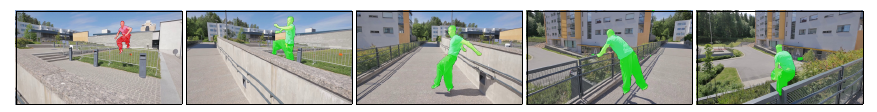
\includegraphics[width=1.0\linewidth]{figures/osvos1.png} 
\caption{ Example result of OSVOS \cite{osvos}: The segmentation of the first frame (red) is used to learn semantics of interested object, whicich is segmented in the rest of the frames independently (green).}
\end{figure}

Caelles et al. \cite{osvos} modified a CNN network pre-trained for image recognition and fine-tuned it for object segementation, as shown in figure 2.2. This was achieved by training it on a set of videos with manually annotated objects. They designed OSVOS by adopting a fully convolutional network (FCN), suitable for dense predictions. The major drawback with use of FCN for task of segmentation is the coarse scale of the deeper layers due to downsampling of feature maps. This leads to inaccurately localized predictions. One way to overcome this drawback is by making use of skip connections of initial larger feature maps \cite{unet}. To avoid this inaccuracy, OSVOS combined information from all network layers to predict segmentation mask for the image. \par

\begin{figure}[h!]\label{fig:osvos1}
\centering
 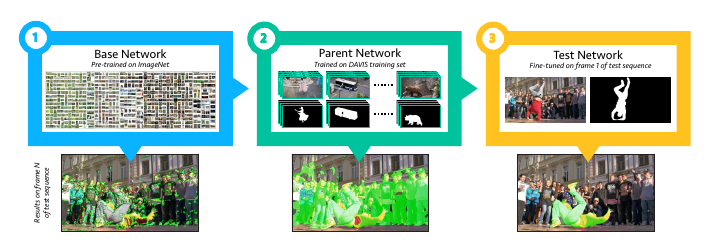
\includegraphics[width=1.0\linewidth]{figures/osvos_train.png} 
\caption{Overview of OSVOS \cite{osvos}: (1) Pre-trained base CNN; its results in terms of segmen-
tation. (2) Training of network for task of object segmentation, parent network. (3) By fine-tuning on a segmentation example for the specific object in first frame, the network rapidly adopts to focus on that target.
}
\end{figure}

 The design of architecture of OSVOS network drew inspiration from the CNN architecture of \cite{maninis:2016}, originally used for biomedical image segmentation of retinal vessles. The OSVOS network was based on the pre-trained VGG \cite{vgg} network. They removed the last fully connected layers and the output from the deeper layers was interpolated to orginal image size. The VGG architecture can be divied into 5 stages, each consisting of groups of convolutional plus Rectified Linear Units (ReLU). Between these  5 stages, pooling operations downscale the feature maps as we go deeper into the network. The output feature maps (before pooling) from stage 2 to 5 are connected using convolutional layer to form separate skip paths. The output feature maps from each skip path are fused linearly and upscaled as required to generate a segmentation mask of same size of original image. They call these masks as "side outputs". In addition, the feature maps from separate paths are are concatenated to construct a volume with information from different levels of layers. Finally, they linearly fuse the volume of feature maps to a single output, called "main output", which has the same dimensions as the image. They computed cross entropy loss using both "main" and "side" outputs. The use of information from all layers enables the network not to loose finer details of the image.



\section{Motivation for using OSVOS}
Once the base network has been modified and trained to perform object segmentation, the parent network can be considered as a pre-trained network for image segmentation. The network is able to learn object semantics and identify various objects in the image. The test network, as shown in figure 2.2, only needs information about object of interest and starts considering rest of image as background. The test network learns about object from a single frame i.e. a single image and generates segmentation mask for all other frames independently. If we consider the 3D volume of slices of liver tissue similar to a video, each slice can be thought of as a frame. Motivated by this similarity, we decided to fine-tune the parent network using few slices and generate the segmentation mask for the whole 3D volume. The liver vesicles in different slices of 3D volume are approximately similar in size and shape, and thus, fine-tuning using few slices can enable the network to learn various features of vesicles. The use of OSVOS fits our problem due to limited availablity of training data. 

\section{Experiment and results}
We annotated liver vesicles of different size and shapes in few randomly chosen slices. These slices were used to fine-tune the parent OSVOS network to target the object of interest. In literature, we can find that network tends to overfit on a relatively small dataset. The use of augmentation helps in generating more data and avoids network from overfitting. We generated more data using cropped and flipped slices for fine-tuning. The segmentation output from CNN trained using 2 slices is also shown in figure 2.1. It can be seen that the OSVOS is able to learn about the features of object and generates a good segmentation mask with accuracy (F-score) of 0.86.\par

\begin{figure}[h!]\label{fig:cnnslices}
\centering
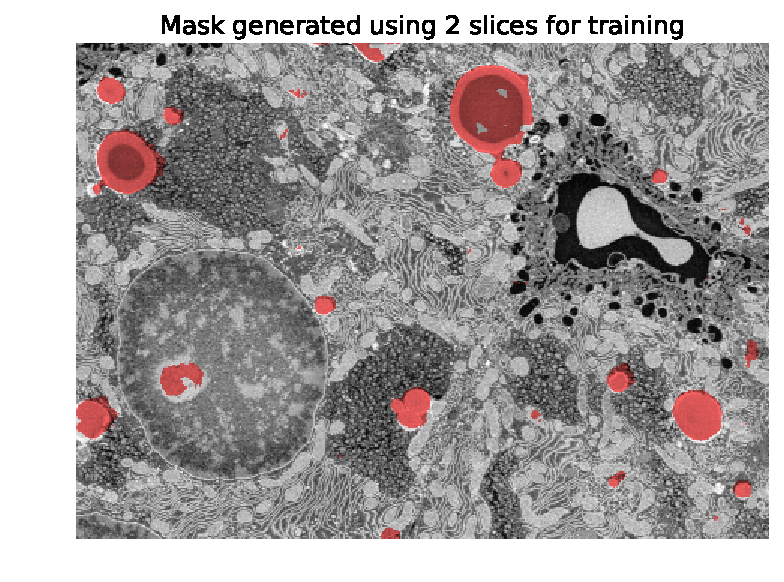
\includegraphics[width=0.9\linewidth]{figures/cnn_mask_2slice.pdf} \\
\caption{Predicted segmentaion mask for part of slice 45}
\end{figure}

In this thesis, we are more interested in observing variation in accuracy with the increase in amount of training data. Thus, we tested OSVOS by fine-tuning it using different number of slices, staring from 1 slice and increasing to 10 slices. For our experiment, set of slice with number \{1,7,10,18,24,52,62,72,80,88\} were used for training. While training, the batch size was always 1. In case of multiple slices i.e. more than 1 slice for training, each slice was fed as separate input to train the network. The set of slices chosen was in ascending order of their number i.e. for training with 3 slices, slice no. \{1,7,10\} were used and for training with 4 slices, slice no. \{1,7,10,18\} were used. These slices were fed to network as an independent image in random order. Once, the parent network was fine-tuned, the test network predicted results for test set. We were not able to test the network on whole 3D volume due to lack of availability of ground truth segmentation mask for whole volume. The test set consisted of part of image from slice number 15, 30 and 45. We had multiple masks annotated by experts for these slices. Even for a single slice, for example 15, we had multiple mask differing from each other annotated by same expert. We generated a reference mask using STAPLE algorithm and computed segmentation accuracy for test slices using these refernce masks. The result of the change in traing data can be seen in figure 2.4.

\begin{figure}[h!]\label{fig:cnnslices1}
\centering
 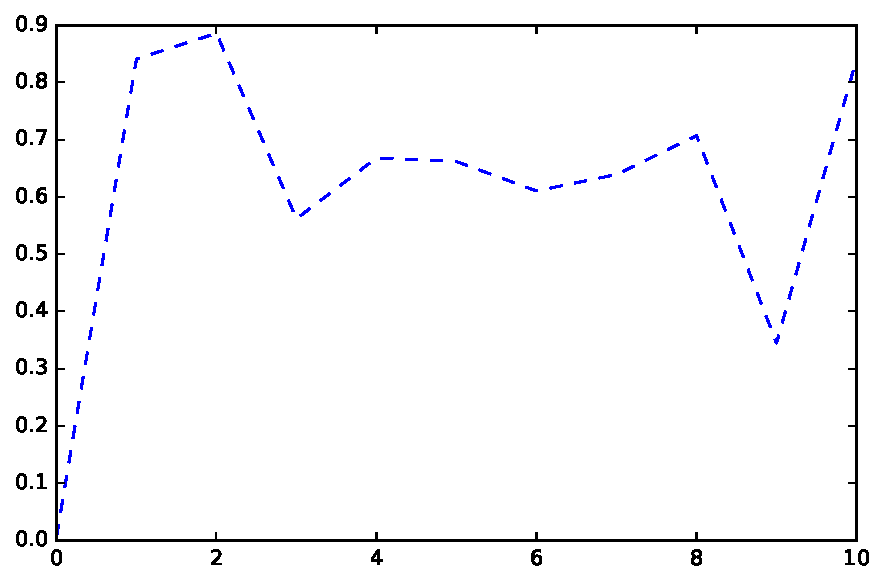
\includegraphics[width=0.9\linewidth]{figures/cnn_diff_slices.pdf} 
\caption{Segmentation accuracy for different amount of training data (Number of slices)}
\end{figure}

We expected an increase in performance with the increase in the amount of training data. This does not happen as CNN is not able to converge equivalently for all cases. We see a significant drop after addition of $9^{th}$ slice, i.e. slice number 80. On analysis, we realized that the training with each slice independently in each forward pass is not allowing the network converge easily with increase in number of slices. Instead, the better way would be to use all available slices in a batch to train the network. Although, we were able to get a significant accuracy with such few annotated slices but it is important to remember here that annotating one slice is not same as annotating one object in a video. We can observe that a single slice contains multiple objects, as shown in figure 2.3. Also, if the experts make few changes in annotated masks used for training, this will force us to train the network again. These difficulties motivated us to try semi-supervised learning using RF for our task of segmentation and try to achieve similar accuracy.


%% ----------------------------------------------------------------------------
% BIWI SA/MA thesis template
%
% Created 09/29/2006 by Andreas Ess
% Extended 13/02/2009 by Jan Lesniak - jlesniak@vision.ee.ethz.ch
%% ----------------------------------------------------------------------------
\newpage
\chapter{Semi-supervised image segmentation}
The philosophy behind semi-supervised learning is to propagate label information from labelled to unlabelled data. Image segmentation can be seen as a classification problem which consists of assigning a class label to each pixel. For our task of binary segmentation, this means classifying each pixel as foreground or background. For our task of image segementaion, we make use of partial annotations as \textit{scribbles}. Scribbles are pixels in image annotated by experts as foreground or background. We use example-based methods to learn from these scribbles annotated by experts. In contrast to having different images for training and testing, we use same image for training and testing as the samples used for training are pixels and not images.

\section{Random Forest}
In this section, we make use of RF as semi-supervised learning algorithm. The advantages and details of using RF can be found in Dominic[cite]. For training RF, we compute set  of features in Python. We compute different features ranging from simple Sobel edge detectors to higher level Gabor filters.The choice of features was made according to WEKA[cite] toolset of FIJI[cite] plugin. These are set of 2D features and perform well medical images. We compute different type of features for a range of sigmas, which gives 65 feature maps for a single image. The details of features computed can be found in Appendix[cite]. In thesis by Dominic, we can find details and effect of feature selection for training Random forests. Here, we focus on how to get best results for given annotation budget and thus, use all features computed and sufficient number of trees to get best results. As shown in figure 4, we can observe that the segmentation measure saturates for more than 50 trees. We try to answer the question of where to scribble and how to make best use of our annotation budget and time.

\subsection{Where to scribble?}
In general, we believe that the more training data we provide, more we can improve the results. Does this hold for partial annotation such as scribbles? If we go on increasing the pixels annotated arbitatrily, will it improve the segmentation mask or we have to use our labelling effort intelligently to improve results? We conducted an experiment by dividing our set of foreground and background scribbles into 2 classes: easy and hard. We classified scribbles as "easy" and "hard" depending on effort required to annotate these pixels. For example, pixels are difficult to annotate near boundary of foreground and background, and we classify these pixels as "hard", as shown in figure 4. First, we trained and tested RF on one image by increasing scribbles belonging to "easy" foreground and background class. The result can be observed in figure 5. \par

We can observe that after [cite] pixels selected from "easy" foreground and background, the segmentation measure do not improve significantly. An improvement can be 

\section{Bayesian Formulation}
We model our image segmentation problem as a Bayesian inference problem.
Let us cosider an observed image, \mat{I} and labeled or segmented groud truth, \mat{S}, the joint probabilty can be defined as:
\begin{equation*}
\p(\mat{I}, \mat{S}) = \p(\mat{S}) \p(\mat{I}|\mat{S}) \eqcont
\end{equation*}
and applying Bayes theorem,
\begin{align*}
\p(\mat{S}|\mat{I}) \, & = \frac{\p(\mat{S}) \p(\mat{I}|\mat{S})}{\p(\mat{I})} \\
						& \alpha \, {\p(\mat{S}) \p(\mat{I}|\mat{S})}
\end{align*}
The left hand side is the probability of \mat{S} given the image \mat{I}, is called the
posterior probability. \p(\mat{S}) is the prior probability of \mat{S}. The Maximum a posteriori (MAP) estimate, $\mat{S^*}$ can be calculated as follow:
\begin{equation}
\mat{S^*} = \arg\max_{\mat{S}}({\p(\mat{S}) \p(\mat{I}|\mat{S})}) \eqend
\end{equation}

The above problem can as well be stated as an energy minimization problem by
writing Equation 3.1 in terms of energy:
\begin{align*}
\funop{E}(\mat{S}) &=\, - \, \log(\p(\mat{I}, \mat{S})) \\
&= -\, \log(\p(\mat{I}|\mat{S})) - \log(\p(\mat{S})) \\
&= \funop{E_d}(\mat{I}, \mat{S}) + \funop{E_r} (\mat{S})
\end{align*}
The total energy, $\funop{E}$, that we want to minimize can be considered as linear combination of data term, $\funop{E_d}$ and prior term (or regularization), $\funop{E_r}$. This modifies calculating MAP estimate to:
\begin{equation*}
\mat{S^*} = \arg\min_{\mat{S}}({\funop{E_d}(\mat{I}, \mat{S}) + \funop{E_r} (\mat{S})}) \eqend
\end{equation*}

\section{Data energy term or Maximum likelihood cost function}
Explain different cost functions

\section{Prediction models}
\subsection{Random Forests}
Explain random forests
\subsection{Convolutional Neural Networks}
Neural networks \newline
Explain transfer learning also.

\section{Prior energy term using Total Variation}
Explain total variation regularisation term.


\chapter{Implementation}
\section{Solving variational problem using ASB}
Solution of ASB problem
\section{Random Forest}
Feature selection and training of Random forests.
\section{Architecture of CNN used}
Training of CNN \newline
Loss function for scribbles

%% ----------------------------------------------------------------------------
% BIWI SA/MA thesis template
%
% Created 09/29/2006 by Andreas Ess
% Extended 13/02/2009 by Jan Lesniak - jlesniak@vision.ee.ethz.ch
%% ----------------------------------------------------------------------------

\chapter{Conclusion}
The aim of this thesis was to analyze the relation between segmentation accuracy and annotation effort. We understood the requirement of iterative semi-interactive annotation to obtain best results for given annotation budget. The semi-interactive process can direct us to obtain best results instead of using our effort arbitrarily in semi-supervised learning. Another thing we tried, were different methods to compensate for training data. We started with the use of pre-trained network using fully annotated objects. It was observed to get good results even with 2 images used for training. Then, we used the Bayesian framework to use variational methods and observe a boost in performance. This motivates us to make use of variational methods to compensate for the lack of data. Finally, we were able to use CNN with variational methods to obtain better results. The simple modification of cross entropy loss for scribbles made it possible to use pre-trained fully convolutional networks. This opens a path to use networks pre-trained on million of images in semi-supervised learning. We also observed that for our given data, RF worked better than CNN in the case of fewer data. This can help in making a choice of method to be used for given annotation budget. \par
Currently, the use of total variation may not be common because of its implementation. It is considered as a post-processing step and not as a solution in a Bayesian framework. In literature, we found recent papers trying to combine CNN and variational methods to obtain better results. They also showed that it can simplify the complexity of CNN and is able to utilize prior information. Ranftl \cite{ranftl:2014} did this by adding total variation as an inference layer and solved the final problem using bilevel optimization \cite{ochs:2015}. This approach has a benefit to learn appropriate regularization parameter ($\lambda$) for total variation. The other approach related to implementation is to split the iterations used to optimize final problem (mentioned in section 3.2) as separate layers in the neural network. This is termed as Primal-dual network and described in Riegler et al. \cite{riegler:2016}. Each iteration can be implemented as one additional layer in networks. We tried to couple these two approaches and came up with the idea of having variational neurons similar to convolution filters. These variational neurons will take the image as input and produce a TV regularized output. Instead of learning $\lambda$, we can use multiple values of $\lambda$ and combine then using a CNN. This also opens a way to remove drawback of finding appropriate $\lambda$, while using variational methods. Due to time restriction, we were not able to complete this, but this idea can provide an option to get best out of multiple methods in a simple unified way. 


%% ----------------------------------------------------------------------------
% If Appendix is needed
% %% ----------------------------------------------------------------------------
% \appendix
% %% ----------------------------------------------------------------------------
% BIWI SA/MA thesis template
%
% Created 09/29/2006 by Andreas Ess
% Extended 13/02/2009 by Jan Lesniak - jlesniak@vision.ee.ethz.ch
%% ----------------------------------------------------------------------------
\chapter{The First Appendix}

In the appendix, list the following material: 

\begin{itemize}
 \item Data (evaluation tables, graphs etc.)
 \item Program code
 \item Further material 
\end{itemize}


%% ----------------------------------------------------------------------------
% Bibliography is stored in references.bib file, and can often be found
% online on webpages like dblp.uni-trier.de
%
% To include it in your thesis, run
%  pdflatex main
%  bibtex main
%  pdflatex main
%  pdflatex main
%
% This ensures all references are done correctly.
%% ----------------------------------------------------------------------------

%\bibliographystyle{plain}
\bibliographystyle{unsrt}
\bibliography{references}

\end{document}

